% !TEX root = ../main.tex
% !TEX spellcheck = en_US
\chapter{Introduction}
Have you ever wanted the bot\footnote{A bot is a computer player that you either can play with or against} you played with in an RTS to communicate or control it to test that strategy that you want to play with your friend when s/he is not available? Then you can continue reading as this thesis is about that, a communicating bot that tells its intentions and why to you, the player, and allows you to control the bot using simple commands like, attack, expand, drop.

Although there exist a new (released less than 5 years ago) few Real-Time Strategy (RTS) games, none of these lets you control your bot in a simple way and at the same time communicates its intentions and reasons to you, at least not to our knowledge. This includes research, where we have yet to find a single subject on communication between human player and bot.

Our focus lies in evaluating if it is worthwhile to do further research in this unexplored area, both for the purpose of researchers and for game developers to help them decide if they shall invest money in a collaborative teammate bot for RTS games.

To familiarize you with RTS games, StarCraft, and collaborative game bots a brief description on all subjects is given below. Once you have basic knowledge of the subjects we will give a thorough background what others have done in closely related subjects. Then a detailed description of the methods we used; this includes implementation on the bot, why it was implement this way, and how it was evaluated. Next the results of our experiments and our conclusions are presented; and finally we present new subjects for future work.

\section{RTS}
An RTS game is a computer game that heavily relies on strategy and fast execution. An analogy would be to play chess where both you and your opponent can move pieces at the same time, you will only see your own pieces and a tile beside them—meaning you do not know the location of the opponent’s pieces or when s/he makes a move—on top of that you have to think of a strategy fast before your opponent gets a lead.

In reality, RTS games resembles more a battle field than a game of chess—you control the army (both units and structures) and what to spend the resources on. At the start of the game you have a single base and your goal is to build up the technology to create powerful units by collecting resources. Often you cannot go straight for the best technology as it takes time and resources to build up all necessary technology and if you only focus on technology you will not have any units for defense if the enemy comes.

In most, if not all, RTS games the player can choose whether s/he wants to play a campaign—usually accompanied with a story—or a simple skirmish game. A skirmish game is in its simplest form a quick battle where both you and your enemy or enemies start with the same amount of resources and structures. Many variants of skirmish games can be played, this thesis will focus on team skirmishes, more specific teams of 2 players versus 2 players. One human collaborating with our proposed teammate bot in one team, and two default bots\footnote{A default bot is the bot that already exists in the game, usually when the player want to play against it during skirmish matches.} in the other team. How this will work is explained throughout the thesis.

There is no real standard for RTS games, they all work a bit different from each other. Instead of covering all different types of RTS games a short description how StarCraft: Brood War works will be given to make the reader familiar with the game before talking about more specific problems and solutions. We choose StarCraft: Brood War because it was the most well-known and widespread RTS game of all time until maybe the introduction of StarCraft 2. More reasons why we chose StarCraft: Brood War can be found in section \ref{sec:why_starcraft}

\subsection{StarCraft}
The AI is implemented in an RTS game: StarCraft, more specifically StarCraft: Brood War—an expansion to StarCraft that introduced new units. Henceforth StarCraft: Brood War will be referenced as StarCraft for simplicity. The StarCraft description below was gathered both from the StarCraft manual\cite{scmanual}, the inofficial StarCraft wiki\cite{scwiki}, and the our observations in gameplay. E.g. to test whether Protoss shields regenerated in battle, we created a single player game where a probe was sent to attack another probe and we observed that shields regenerates in battle since the probe’s shield points regenerated (increased). Figure \ref{fig:starcraft} shows a print screen of a Terran base from one of the campaign maps.

\begin{figure}[htb]
\centering
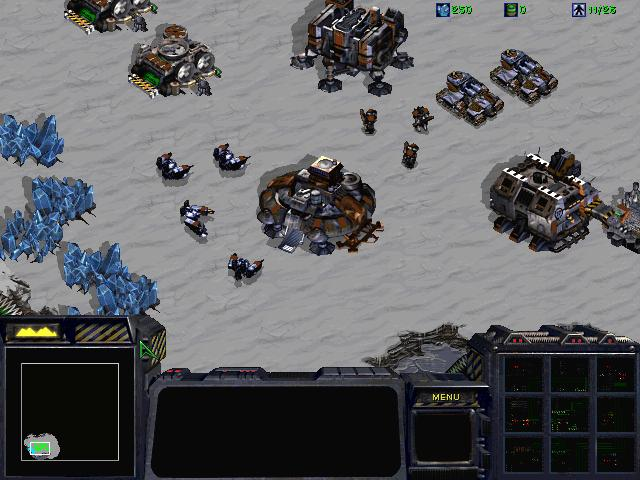
\includegraphics[width=0.8\textwidth]{starcraft}
\caption{Print screen from StarCraft.}
\label{fig:starcraft}
\end{figure}

\subsubsection{Gameplay}
StarCraft has three races—Terran, Protoss, and Zerg—which the player can choose from. Each of these races have their own unique types of units and varying play styles.

\paragraph{Commonalities between races}
All races have worker units that collect minerals and gas—minerals and gas are game resources used to build structures, units and upgrades. Minerals and gas are usually located in clusters of several mineral fields and occasionally a Vespene geyser (gas). The player always starts at a base with both mineral fields and a Vespene geyser. To mine minerals and gas, workers go to the fields and then return to the closest main structure of the player. Because of the travel distance you usually want to build a new main structure near resource clusters.

Mineral fields have a fixed number of resources they can yield; when all have been depleted the mineral field disappears. A Vespene geyser on the other hand does not disappear after depletion, instead each worker now brings back 2 units of gas each turn, instead of 8. To be able to mine gas in the first place a structure needs to be placed on a Vespene geyser. Only one worker can simultaneously collect minerals from a mineral field, or gas from a gas depot, other workers are automatically queued to start mining when the first worker brings back the resources.

\label{sec:starcraft_supply}
StarCraft limits the number of units one can have to 200 supply\footnote{Called Psi for Protoss, and Control for Zerg which makes more sense on those unit. Supply is, however, the most common used jargon for all races.}. Each unit occupies some supply, ranging from a half supply (Zerglings) to six supplies (Carriers), armed nuclear silos take up 8 supplies. In general, the better the unit the more supply it occupies. The player starts with 9 to 10 max supply (depending on the race). To increase the max supply a special structure (unit for Zerg) can be built; main bases also generate supply, 10 for Terran Command Center, 9 for Protoss Nexus, and 1 for Zerg Hatchery.

\paragraph{Constructing Structures}
When Terran's worker unit, SCV, constructs a structure it becomes occupied and cannot do anything else; the SCV can however be targeted, and can stop building and let another SCV take over—e.g. when an enemy starts attacking the SCV.

Zerg’s worker unit, Drone, will morph itself into a structure. The drone will disappear once the morphing stage begins, but if the player cancels the building progress the drone will reappear. Once the morph completes the drone is forever lost. Zerg structures need to be placed on creep which Hatcheries and colonies help to spread; exceptions are Hatcheries and Extractors (for Vespene Geyser).

Protoss’s worker unit, Probe, need to construct structures in a psionic power grid, a circle grid generated by Pylon structures; exceptions are Nexuses, Pylons, and Refineries (for Vespene geyser). If a structure becomes unpowered it will stop functioning until a nearby Pylon is reconstructed to create a new psionic power grid. Once a structure has been planted, it will construct itself leaving the Probe free for other tasks.

\paragraph{Constructing Units}
Terran and Protoss function in basically the same way: they both have separate unit producing structures for different kinds of units, e.g. Barracks/Gateway for basic ground units, Starport/Stargate for flying units, and so forth. All units, however, cannot be built from these structures directly, some units require another stand-alone structure, like Acadamy for Firebats and Medics. The main structure (Command Center and Nexus) can only build workers. Only one unit can be built simultaneously from these structures, if one wants a huge production of units, large amounts of unit producing structures are needed.

Zerg on the other hand only has one unit producing structure, the Hatchery, that pops out larvae in a certain time interval—one Hatchery can maximum have three larvae. These larvae can be morphed into the unit of choice. To build other units than Drones and Overlords the player must build the structure needed for the unit, e.g. building a Spawning Pool to be able to morph Zerglings from a larvae, in a similar way Academy is needed for building Firebats from a Barracks. This makes Zerg good for creating lots of better units with a minimum extra cost, because it only needs one extra building and some Hatcheries. E.g. if Zerg has 3 Hatcheries it can save its larva and when the new building is complete it can directly start producing 9 of the new units. Whereas Terran needs to build 9 Barracks, Factories, or Starports (depending on the unit) to have the same rate of production.

While it seems most obvious to build “the best” units at the beginning, this is not possible—although there is no such thing as best unit as all units are good depending on the situation, powerful unit might be a better wording. A powerful unit require certain structures, that in turn require other structures, i.e. unit and structure requirements can be seen as an acyclic graph  where the best structures and units are at the ends. For example, to build a Carrier one requires a Fleet Beacon (for the Carrier tech) and a Stargate (to build the unit), the Stargate then requires a Cybernetics core, the Cybernetics core requires a Gateway and a Gateway requires a Nexus. As you might conclude, you need a lot of resources and time to be able to build a Carrier; if you go straight for Carriers your enemy can just waltz into the base with any number of units and kill the entire base.

\paragraph{Unit Health}
The health of units for each race works a bit different. Terran units do not generate health. Mechanical units (both ground and air) and structures can be repaired by an SCV at the cost of minerals and gas, depending on what resources were required to build the unit or structure; an SCV can also repair another SCV since they are vehicles. Biological units, such as marines and medics can only restore lost hit points (HP) by medics which have a healing ability that restores 2 HP per 1 energy; this ability can be cast every second. In addition medics have the ability to heal Protoss and Zerg biological units—which makes Terran a good team race.

Protoss units are a bit special, they have two health bars, one for health the other for shields. These are usually divided by half, meaning units have equal amount of health as shields, an exception is Archons which have 10 HP and 350 shield points (SP). Shields regenerate much faster than zerg’s regeneration ability, including in battle, but always takes full damage from all damage types. Terran Science Vessels can drain all the shield instantly through its EMP ability. Shields can, however, be fully recharged by a protoss support structure, shield battery, which converts its energy to shields, just as medics can heal biological units.

All Zerg units and structures automatically regenerates health at a very slow rate, even during battle, but because it regenerates slowly units usually only heal 1 or 2 HP during a shorter battle.

\section{Teammates}
A teammate is a player, either human or bot, that helps the team towards a common goal. Teammate bots often prioritize the human player because it is their experience, thus the bot acts as a helper to the player and team.

\subsection{Human teammate}
You can divide human teams into essentially two groups: where players more or less cooperate with each other and teams whose players “do their own thing” not caring about what the others do. Although the reality is more a gray scale, often players do not only cooperate or only do their own thing, but instead it varies throughout the gameplay.

Humans are good at forming complex strategies, or at least complex to program an AI to understand what to do. They can come and aid their teammate intuitively without the teammate asking for help.

When playing together with other humans, communication is important. If verbal communication is possible, players can tell their intentions to the teammates—e.g. attacking, defending, moving—other important game changes—e.g. enemy missing, getting shot, spotting an enemy—or just requesting help. When the player cannot communicate verbally, text messages through the games are often possible, but this can disrupt gameplay since actions are often disabled while typing (depending on the game). Short text messages are often sent instead to convey the entire message; e.g. “attack” instead of “I’m going to attack the enemy base from this side, join me.” 

\paragraph{StarCraft}
In StarCraft, players that know each other usually decide what strategy to use before starting the game, whereas if the players do not know each other they can discuss a common strategy to use, announce their strategies, or both. If verbal communication is possible, players like to talk about tactics during the game, they like to convey their intentions to the teammate player.

\subsection{AI teammate}
A general teammate bot tries to replace a human player. In some games they are used to replace an ideal human player. This bot usually tries to figure out what the player is doing and either figure out a strategy that works with this or trying to deduct what the player want bot to do. When a bot works, it feels like a human player, especially if the game provides some sort of communication to the player. If you, however, have played a game where the bot breaks, you can feel that it is mechanical.

In other games teammate bots only have a minor role; in Modern Warfare 2\cite{callofduty}, a first-person shooter (FPS), you have teammate bots helping you in certain areas, these bots do not do much, but are there for the player. They do, however, “cooperate” with the player—we say “cooperate” because the bots usually only follow the player while making sure behaving accordingly such as avoiding places between the player and his/her target.

\paragraph{StarCraft}
The standard AI in StarCraft probably does not have any specific AI when it plays a cooperative game with a human player; as it does not interact with the player and acts on its own, neither helping the player nor taking help from the player. 